\documentclass[t]{beamer}

\subtitle{Section 2.7: Groups of Motions and Symmetries}

\input{../../_tools/setup}

\begin{document} 
	\startdoc
	
	\topics{
		\item Cosets 
		\item Lagrange's Theorem
		\item Corollaries to Lagrange!
	}{
		\item Dihedral Groups
		\item Groups of order 2p
	}



\begin{frame}[fragile]
	\frametitle{\fn}
	\begin{defn}
		A \emph{regular $n$-gon} is an $n$-sided polygon whose sides are all congruent.  Denote this figure by $P_n$.
	\end{defn}
	\begin{exa}
		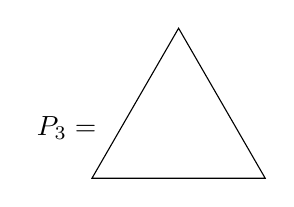
\begin{tikzpicture}
	\draw (90:.5in) \foreach \x in {210,330} {
		-- (\x:.5in)
	} -- cycle;
	\node[xshift=-.56 in] {$P_3=$} ;
	\end{tikzpicture}\hfill
	\begin{tikzpicture}
	\draw (45:.5in) \foreach \x in {135,225,315} {
		-- (\x:.5in)
	} -- cycle;
	\node[xshift=-.56 in] {$P_4=$} ;
	\end{tikzpicture}\hfill
	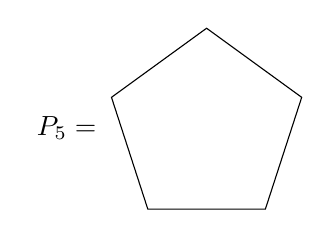
\begin{tikzpicture}
	\draw (90:.5in) \foreach \x in {162,234,306,18} {
		-- (\x:.5in)
	} -- cycle;
	\node[xshift=-.7 in] {$P_5=$} ;
	\end{tikzpicture}
	\end{exa}
\end{frame}

\slide{
	\begin{defn}
		A \emph{symmetry} of $P_n$ is any action on $P_n$ by a sequence of flips and/or rotation which return $P_n$ to its original position in the plane.
	\end{defn}

	\begin{defn}
		The \emph{dihedral group} $D_n$ is the group of symmetries of the figure $P_n$.  (Operation is composition.)
	\end{defn}

	\begin{nb}
		And now we move on to the worksheet.
	\end{nb}
}


%\begin{frame}[fragile]
%	\frametitle{\fn}
%		\begin{statementblock}{Claim}
%		The group of symmetries of an equilateral triangle is generated by a flip and a $120^\circ$ rotation.
%	\end{statementblock}
%	\begin{block}{\textbf{Notation.}}
%		We'll use $f$ to denote the flip across the vertical axis and $r$ to be rotation by $120^\circ$ clockwise.
%		\begin{center}
%			
%		\begin{tikzpicture}
%			\draw (90:.35in) \foreach \x in {210,330} {
%				-- (\x:.35in)
%			} -- cycle;
%			\node at (90:.15in) {3};
%			\node at (210:.15in) {2};
%			\node at (330:.15in) {1};
%			\draw[xshift=.5in] (180:.25in) -- (0:.25in) (0,0) node[above] {$f$} (0:.25) node[right] {$>$};
%			\draw[xshift=1in] (90:.35in) \foreach \x in {210,330} {
%				-- (\x:.35in)
%			} -- cycle;
%			\node[xshift=1in] at (90:.15in) {3};
%			\node[xshift=1in] at (210:.15in) {1};
%			\node[xshift=1in] at (330:.15in) {2};
%		\end{tikzpicture}
%		\quad \quad \quad
%		\begin{tikzpicture}
%			\draw (90:.35in) \foreach \x in {210,330} {
%				-- (\x:.35in)
%			} -- cycle;
%			\node at (90:.15in) {3};
%			\node at (210:.15in) {2};
%			\node at (330:.15in) {1};
%			\draw[xshift=.5in] (180:.25in) -- (0:.25in) (0,0) node[above] {$r$} (0:.25) node[right] {$>$};
%			\draw[xshift=1in] (90:.35in) \foreach \x in {210,330} {
%				-- (\x:.35in)
%			} -- cycle;
%			\node[xshift=1in] at (90:.15in) {2};
%			\node[xshift=1in] at (210:.15in) {1};
%			\node[xshift=1in] at (330:.15in) {3};
%		\end{tikzpicture}
%		\end{center}
%	\end{block}
%	
%	\begin{nb}
%		The book uses $a$ for $r$ and $b$ for $f$. I like to use $\sigma$ for $r$ and $\tau$ for $f$.
%	\end{nb}
%\end{frame}
%
%\begin{frame}[fragile]
%	\frametitle{\fn}	
%	\begin{nb}
%		We can think of the symmetries of the regular triangle as an element of $S_3$.
%	\end{nb}
%	\begin{center}
%		\begin{minipage}{1.5in}
%			\begin{tikzpicture}
%			\node[smaller]{};
%			\node at (90:.65in) {\color{blue} 3};
%			\node at (210:.65in) {\color{blue} 2};
%			\node at (330:.65in) {\color{blue} 1};
%			\node at (90:.25in) {\color{red} 2};
%			\node at (210:.25in) {\color{red} 1};
%			\node at (330:.25in) {\color{red} 3};
%			\end{tikzpicture}
%		\end{minipage}
%		\begin{minipage}{1.5in}
%			$\leftrightarrow$\quad
%			$\ds r= \begin{pmatrix}
%			\color{red} 1&\color{red} 2&\color{red} 3\\
%			\color{blue}2&\color{blue} 3&\color{blue} 1
%			\end{pmatrix}$
%		\end{minipage}
%	\end{center}
%\end{frame}
%
%\slide{
%	$$\large \begin{array}{|c|c|c|p{1.25in}|p{1in}|}
%	\hline
%	\text{Elt}&\text{Two-line}&\text{cycle}&Symmetry&Picture\\\hline
%	e&\begin{pmatrix}
%	1&2&3\\1&2&3
%	\end{pmatrix}&\varepsilon&do nothing&\\\hline
%	r&\begin{pmatrix}
%	1&2&3\\2&3&1
%	\end{pmatrix}&(1\ 2\ 3)&$120^\circ$ clockwise&\\\hline
%	r^2&\begin{pmatrix}
%	1&2&3\\&&
%	\end{pmatrix}&&&\\\hline
%	f&\begin{pmatrix}
%	1&2&3\\&&
%	\end{pmatrix}&&&\\\hline
%	fr&\begin{pmatrix}
%	1&2&3\\&&
%	\end{pmatrix}&&&\\\hline
%	fr^2&\begin{pmatrix}
%	1&2&3\\&&
%	\end{pmatrix}&&&\\\hline
%	\end{array}
%	$$
%}
%
%\slide{
%	\begin{exercise}
%		 Did we miss any other symmetries? Why or why not? Is this set of symmetries equal to $S_3$?
%	\end{exercise}\vskip 1in
%	\begin{exercise}
%		Use your cut-out triangle to find the symmetry $r^2frf^3r^4f$, in 2-line notation $\ds\begin{pmatrix}
%		1&2&3\\&&
%		\end{pmatrix}$.
%	\end{exercise}
%}
%\slide{
%	\begin{exercise}
%		Use your cut-out triangle to prove that $f^2=e$, $r^3=e$, and $frf=r^2$.
%	\end{exercise}\vskip .5in
%	 \begin{exercise}
%	 	Use the identities in question 3 to reduce $r^2frf^3r^4f$ to $r^2f$.  Can you use an identity to make $r^2f$ look like one of the 6 symmetries in the table?
%	 \end{exercise}
%}
%\begin{frame}[fragile]
%	\frametitle{\fn\ - On to Squares}
%	\begin{center}
%		\begin{minipage}{1.5in}
%			\begin{tikzpicture}
%			\node[smsquare]{};
%			\node at (45:.65in) {\color{blue} 4};
%			\node at (135:.65in) {\color{blue} 3};
%			\node at (225:.65in) {\color{blue} 2};
%			\node at (315:.65in) {\color{blue} 1};
%			\node at (45:.25in) {\color{red} 3};
%			\node at (135:.25in) {\color{red} 2};
%			\node at (225:.25in) {\color{red} 1};
%			\node at (315:.25in) {\color{red} 4};
%			\end{tikzpicture}
%		\end{minipage}
%		\begin{minipage}{1.75in}
%			$\leftrightarrow$\quad
%			$\ds r= \begin{pmatrix}
%			\color{red} 1&\color{red} 2&\color{red} 3&\color{red}4\\
%			\color{blue}2&\color{blue} 3&\color{blue} 4&\color{blue} 1
%			\end{pmatrix}$
%		\end{minipage}
%	\end{center}
%\end{frame}
%\slide{\vskip -.1in\hspace*{-.25in}
%	$ \begin{array}{|c|c|c|p{1.25in}|p{1in}|}
%	\hline
%	\text{Elt}&\text{Two-line}&\text{cycle}&Symmetry&Picture\\\hline
%	e&\begin{pmatrix}
%	1&2&3&4\\1&2&3&4
%	\end{pmatrix}&\varepsilon&do nothing&\\\hline
%	r&\begin{pmatrix}
%	1&2&3&4\\2&3&4&1
%	\end{pmatrix}&(1\ 2\ 3\ 4)&$90^\circ$ clockwise&\\\hline
%	r^2&\begin{pmatrix}
%	1&2&3&4\\&&
%	\end{pmatrix}&&&\\\hline
%	r^3&\begin{pmatrix}
%	1&2&3&4\\&&
%	\end{pmatrix}&&&\\\hline
%	f&\begin{pmatrix}
%	1&2&3&4\\&&
%	\end{pmatrix}&&&\\\hline
%	fr&\begin{pmatrix}
%	1&2&3&4\\&&
%	\end{pmatrix}&&&\\\hline
%	fr^2&\begin{pmatrix}
%	1&2&3&4\\&&
%	\end{pmatrix}&&&\\\hline
%	fr^3&\begin{pmatrix}
%	1&2&3&4\\&&
%	\end{pmatrix}&&&\\\hline
%	\end{array}
%	$
%}
%
%\slide{
%	\begin{block}{\textbf{Brain Break.}}
%		Do you prefer
%		\enumarabic{
%			\item chocolate candy?
%			\item fruity candy?
%		}
%	\end{block}
%}

\slide{
\begin{defn}
	Let $n\geq 2$.  The \emph{dihedral group} $D_n$ is the group of order $2n$ presented as follows:
	
		\[D_n=\{e,r,r^2,\dots,r^{n-1},f,fr,fr^2,\dots,fr^{n-1}\},\]
	where $|r|=n$, $|f|=2$, and $r f=fr^{-1}$.
\end{defn}
\begin{nb}
	The last relation $rf=fr^{n-1}$ can be written in many other ways, such as
	\bulletize{\item $frf=r^{n-1}$\item $rfr=f$ ({\color{orange} this is the one the book uses})\item $r^if=fr^{-i}$ for all $i\in\Z$\item $fr^if=r^{-i}$ for all $i\in\Z$\item $r^ifr^i=f$ for all $i\in\Z$}
\end{nb}
}
%\slide{\begin{exercise}
%	Let $r,f$ be elements of any group $G$ satisfying $|r|=e$ and $|f|=2$. Prove that $$rfr=f\Leftrightarrow frf=r^{n-1}.$$
%\end{exercise}
%\begin{exercise}
%Let $r,f$ be elements of any group $G$ satisfying $|r|=n$ and $|f|=2$. Prove that $$frf=r^{n-1}\Leftrightarrow fr^if=r^{-i}.$$
%\end{exercise}}
\slide{
	\begin{nb}
		Here's the generator notation for $D_n$:
			\[D_n=\left.\left\langle f,r\ \right|\ f^2=e,r^n=e, rf=fr^{-1}\right\rangle.\]
	\end{nb}
}

%\slide{
%	\begin{thm}{2.6.3 (sorta)}
%		Let $G$ be a group of order 6. Then $G$ is cyclic, or $G\cong D_3$.
%	\end{thm}
%%	\begin{block}{Proof.}
%%		Let $G$ be a group with $|G|=6$.  Assume $G$ is not cyclic. We want to show $G\cong D_3$.  Since $G$ is not cyclic, $|g|<6$ for all $g\in G$.  And so by a Corollary to Lagrange's Theorem $|g|=1,2,$ or $3$.
%%	\end{block}
%}

%\slide{
%	\begin{block}{Proof of Thm 2.6.3 (Cont.)}
%	\textbf{Claim.} $G$ has an element of order 3.\\
%		\mbox{}\hspace*{.25in}
%		\begin{minipage}{.85\textwidth}
%			\begin{proof}[Proof of Claim.]
%			Assume toward contradiction that $G$ has no elements of order 3.  Then $g^2=e$ for all $g\in G$, as every $g$ has order 1 or 2.
%			
%			Thus $G$ is abelian. (See section 2.2 Exercise 20.) And so the subset $H=\{e,a,b,ab\}$ with $a\neq b$ non-idenity elements of $G$ is in fact a subgroup of $G$. This is a contradiction as $|H|=4$ does not divide $|G|=6$.
%			\end{proof}
%		\end{minipage}
%	\end{block}}
%
%\slide{
%\begin{block}{Proof of Thm 2.6.3 (Cont.)}
%	Let $r\in G$ be an element of order 3, which now we know exists.  And write $H=\langle r\rangle=\{1,r,r^2\}\leq G$.\\
%	\textbf{Claim.} If $x\in G$ and $x\not\in H$, then $|x|=2$.\\
%		\mbox{}\hspace*{.25in}
%		\begin{minipage}{.85\textwidth}
%			\begin{proof}[Proof of Claim.]
%				Let $x\in G$ and $x\not\in H$.  Notice that since $|G:H|=6/3=2$, $G=H\cup Hx$. Moreover, since $x=x^2x^{-1}\not\in H$, the corresponding cosets are distinct, $Hx\neq Hx^2$, and $x^2\not\in Hx$. Thus $x^2\in H$.    
%				
%				If $|x|=3$, then $x=x^4=(x^2)^2\in H$, contradicting the fact that $x\not\in H$.  Thus $|x|\neq 3$.  Further $|x|\neq 1$, so $|x|=2$.
%			\end{proof}
%		\end{minipage}
%\end{block}}
%
%\slide{
%\begin{block}{Proof of Thm 2.6.3 (Cont.)}
%	Fix some $f\in G$ such that $f\not\in H$. \fbox{why does $f$ exist??}  Then $f^2=e$ by the second claim.  Therefore $G=H\cup fH$, so
%		\[G=\{e,r,r^2,f,fr,fr^2\},\]
%	with $|r|=3$ and $|f|=2$. 
%	
%	Lastly, to show $G\cong D_3$, we must show $frf=r^2$.
%	Since $fr\not\in H$, we know from claim 2 that $(fr)^2=e$.  Hence
%		\[frfr=e\Rightarrow (frf)(rr^2)=r^2\Rightarrow frf=r^2.\]
%\end{block}}
\slide{
	\begin{thm}{2.6.3}
		Let $G$ be a group and $p$ a prime.  If $|G|=2p$, then $G$ is cyclic or $G\cong D_p$.
	\end{thm}
}
%\slide{
%	\begin{exercise}
%		What are ALL groups (up to isomorphism) of orders 1 through 7?
%		$$\begin{array}{|c|c|}
%		\hline
%		|G|&$G$\\\hline\hline
%		1&\hspace*{2in}\\[.5em]\hline
%		2&\\[.5em]\hline
%		3&\\[.5em]\hline
%		4&\\[.5em]\hline
%		5&\\[.5em]\hline
%		6&\\[.5em]\hline
%		7&\\[.5em]\hline
%		\end{array}$$
%	\end{exercise}
%}
\slide{
	\begin{exa}
		The subgroups of $D_4=\{e,r,r^2,r^3,f,fr,fr^2,fr^3\}$.
		\bulletize{
			\item Subgroups of order 4: $\langle r^2,f\rangle$, $\langle r\rangle$, and $\langle r^2,fr^3\rangle$\\
			 \textbf{Exercise.} Which of these are $C_4$, which are $K_4$?
			\item Subgroups of order 2: $\langle f\rangle$, $\langle fr^2\rangle$, $\langle r^2\rangle$, $\langle fr^3\rangle$, $\langle fr\rangle$, 
			\item Subgroup of order 1: $\{e\}$
		}
	\end{exa}
}
\begin{frame}[fragile]
	\frametitle{\fn}
	\begin{exa}
		The full subgroup lattice of $D_4$.
		\begin{center}
		\begin{tikzcd}
	&&D_4\arrow[-]{dll}\arrow[-]{d}\arrow[-]{drr}\\
	\langle r^2,f\rangle\arrow[-]{d}\arrow[-]{dr}\arrow[-]{drr}
	&&\langle r\rangle\arrow[-]{d}
	&&\langle r^2,fr^3\rangle\arrow[-]{dll}\arrow[-]{dl}\arrow[-]{d}\\
	 \langle f\rangle\arrow[-]{drr}
	 &\langle fr^2\rangle\arrow[-]{dr}
	 &\langle r^2\rangle\arrow[-]{d}
	 &\langle fr^3\rangle\arrow[-]{dl}
	 &\langle fr\rangle\arrow[-]{dll}\\
	 &&\{e\}
	\end{tikzcd}
	\end{center}
	\end{exa}
\end{frame}
\end{document}

